% Reading the Trail -- final presentation (6-8 min video).
% Build:  cd video && latexmk -pdf slides.tex
%
% FILLING IN RESULTS
%   * Every number still to be filled is written as \tbd  (grep -n '\\tbd' slides.tex).
%   * Result figures/tables are pulled from ../results automatically once they exist
%     (scripts/analyze.py and scripts/gallery.py); until then a grey placeholder box is shown.
%   * Set the run/split used for the confusion matrix and the gallery here:
\edef\cmrun{\detokenize{e7_ce_dice_s1}}  % final config (E7 = CE+Dice, chosen on val); seed-1 replicate, see paper Sec. III
\edef\cmsplit{\detokenize{test}}
\providecommand{\resultsdir}{../results}

\documentclass[aspectratio=169,11pt]{beamer}
\usetheme[progressbar=frametitle,numbering=fraction,sectionpage=none]{metropolis}
\usepackage[T1]{fontenc}
\usepackage{booktabs}
\usepackage{graphicx}
\usepackage{adjustbox}
\usepackage{xcolor}
\usepackage{tikz}

% ---------------------------------------------------------------- colors
\definecolor{trail}{HTML}{2E5E3E}     % forest green
\definecolor{hazard}{HTML}{C0392B}    % brick red, used sparingly for safety classes
\definecolor{muted}{HTML}{6B7280}
\definecolor{tbdred}{HTML}{D7263D}
\setbeamercolor{frametitle}{bg=trail,fg=white}
\setbeamercolor{progress bar}{fg=hazard,bg=trail!30}
\setbeamercolor{title separator}{fg=hazard}
\setbeamercolor{alerted text}{fg=hazard}
\setbeamerfont{frametitle}{size=\Large}
\setbeamertemplate{itemize items}{\textcolor{trail}{\textbullet}}
\metroset{block=fill}
\setbeamercolor{block title}{bg=trail!15,fg=trail}
\setbeamercolor{block body}{bg=trail!6}

% ---------------------------------------------------------------- helpers
% \tbd marks a number that must be filled in from the results.
\newcommand{\tbd}{{\color{tbdred}\textbf{TBD}}}
% \placeholder[width]{height}{text}: grey box shown while a figure does not exist yet.
\newcommand{\placeholder}[3][\linewidth]{%
  \begin{tikzpicture}
    \node[draw=muted,dashed,fill=muted!8,text=muted,align=center,
          minimum width=#1,minimum height=#2,text width=#1-8mm,font=\small] {#3};
  \end{tikzpicture}}
% \resultfig[includegraphics opts]{file under \resultsdir/figures}{placeholder height}{placeholder text}
\newcommand{\resultfig}[4][width=\linewidth]{%
  \edef\rfname{#2}%
  \IfFileExists{\resultsdir/figures/\rfname}%
    {\includegraphics[#1]{\resultsdir/figures/\rfname}}%
    {\placeholder{#3}{\textbf{Placeholder:} #4\\[2pt]\adjustbox{max width=\linewidth}{\tiny\texttt{results/figures/\expandafter\detokenize\expandafter{\rfname}}}}}}
\makeatletter
\newcommand{\rtstripopt}{\@ifnextchar[{\rt@gobble}{}}
\def\rt@gobble[#1]{}
\makeatother
% Input a booktabs table written by scripts/analyze.py (table*/table float stripped, scaled to fit).
\newcommand{\resulttable}[4]{%
  \IfFileExists{\resultsdir/tables/#1}%
    {\begingroup
       \expandafter\let\csname table*\endcsname\rtstripopt\expandafter\let\csname endtable*\endcsname\relax
       \let\table\rtstripopt\let\endtable\relax
       \renewcommand{\caption}[1]{}\renewcommand{\label}[1]{}\renewcommand{\centering}{}%
       \begin{adjustbox}{max width=#2,max totalheight=#3,center}\input{\resultsdir/tables/#1}\end{adjustbox}%
     \endgroup}%
    {\placeholder[#2]{#3}{\textbf{Placeholder:} #4\\[2pt]\scriptsize\texttt{results/tables/\detokenize{#1}}}}}
\newcommand{\cls}[1]{\textit{#1}}
\newcommand{\takeaway}[1]{\par\vspace{3pt}{\color{trail}\rule{\linewidth}{0.6pt}}\par\vspace{1pt}{\large #1}}

\title{Reading the Trail}
\subtitle{Off-Road Terrain Analysis with Deep Convolutional Networks}
\author{Callen Nash \quad\textcolor{muted}{model \& documentation lead}\\
        Xander Navojosky \quad\textcolor{muted}{data \& evaluation lead}}
\institute{Colorado School of Mines \textperiodcentered{} Deep Learning, final project}
\date{}

\begin{document}

% =================================================================== 1
\maketitle

% =================================================================== 2
\begin{frame}{Why off-road perception is hard}
\begin{columns}[T]
\column{0.55\textwidth}
\begin{itemize}\setlength\itemsep{6pt}
  \item City driving models lean on lanes, curbs, and signs.\\
        \textcolor{muted}{Trails have none of these.}
  \item Grass, mulch, and gravel blend into each other.
  \item Shade, glare, and a shaking camera.
  \item Robots that need it: search and rescue, farming and forestry, planetary rovers.
\end{itemize}
\column{0.42\textwidth}
\vspace{4pt}
\begin{block}{Our question}
Can a network label every pixel of a trail image, \alert{including the rare hazards} (water, logs, rock)?
\end{block}
\end{columns}
\takeaway{Mistaking water for dirt can leave a vehicle stuck or damaged.}
\end{frame}

% =================================================================== 3
\begin{frame}{Task and data: RUGD semantic segmentation}
\centering
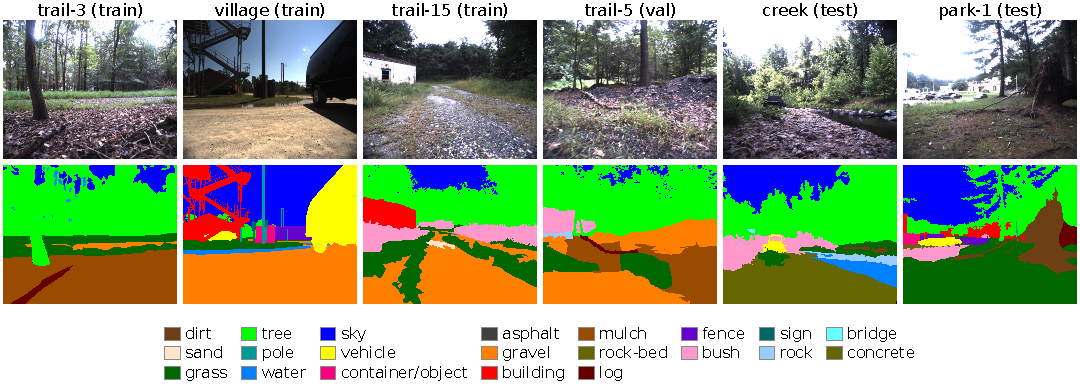
\includegraphics[width=0.94\textwidth]{../results/figures/sample_grid.pdf}\\[4pt]
\small
7,436 labeled frames \textperiodcentered{} 18 video sequences \textperiodcentered{} 24 classes \textperiodcentered{} 688\,$\times$\,550 px, small robot\\[2pt]
Split by sequence: \textbf{4,779 / 733 / 1,924}, so near-duplicate frames never cross splits
\end{frame}

% =================================================================== 4
\begin{frame}{The imbalance problem}
\begin{columns}[c]
\column{0.40\textwidth}
\centering
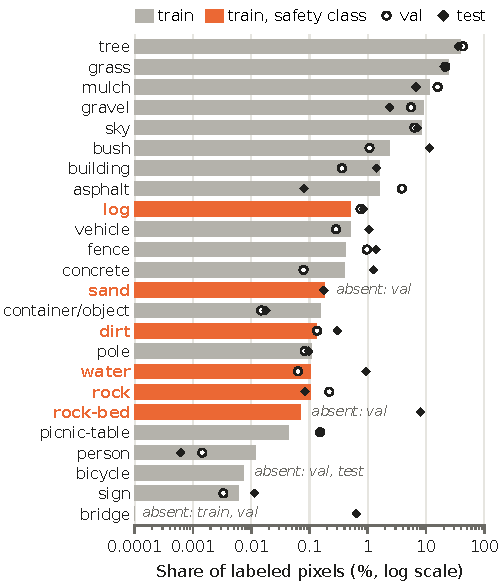
\includegraphics[height=0.80\textheight]{../results/figures/class_frequency.pdf}
\column{0.57\textwidth}
\begin{itemize}\setlength\itemsep{8pt}
  \item \cls{tree} + \cls{grass} cover \textbf{63\%} of training pixels.
  \item Most / least common class: \textbf{6,382\,:\,1}.
  \item Safety classes (\cls{water}, \cls{log}, \cls{rock}, \cls{rock-bed}, \cls{dirt}, \cls{sand}):
        \alert{\textbf{1.1\%} of training pixels}.
  \item Water appears in only \textbf{1 in 13} training frames.
\end{itemize}
\takeaway{A model can score well and still miss every hazard.}
\end{columns}
\end{frame}

% =================================================================== 5
\begin{frame}{Distribution shift: the test split is different}
\begin{columns}[c]
\column{0.63\textwidth}
\centering
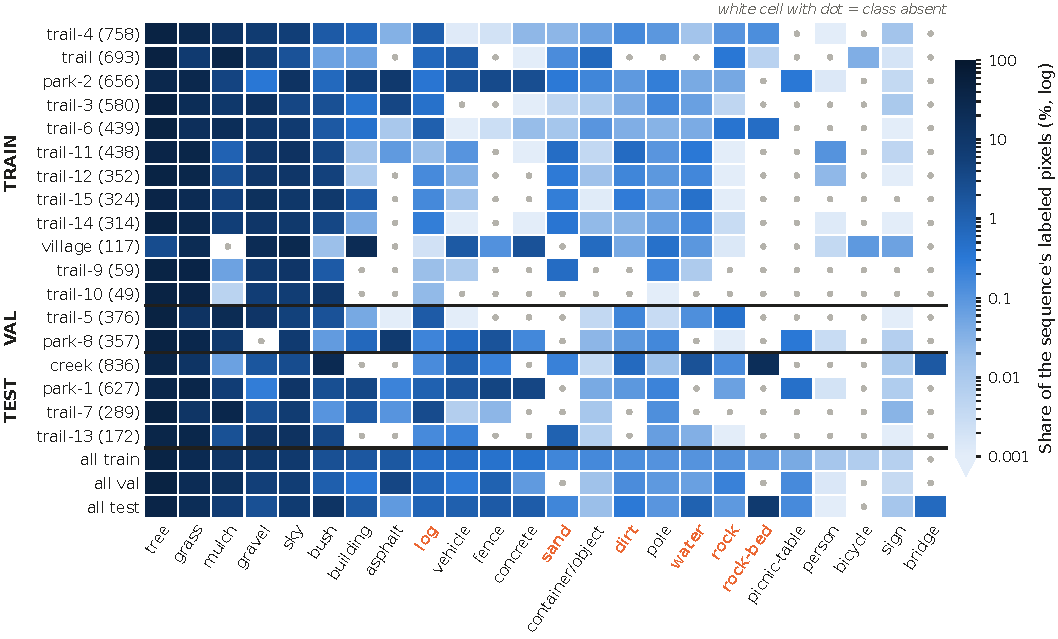
\includegraphics[width=\linewidth]{../results/figures/sequence_class_heatmap.pdf}
\column{0.35\textwidth}
\small
\begin{itemize}\setlength\itemsep{2pt}
  \item Safety classes: \textbf{1.1\%} of train, \alert{\textbf{10.3\%}} of test.
  \item \cls{rock-bed}: 114$\times$ more common in test. Almost all of it is in one sequence, \cls{creek}.
  \item \cls{bridge}: 0 training pixels, 4.6\,M test pixels.
  \item Validation lacks 4 classes.
\end{itemize}
\takeaway{\normalsize Expect validation scores to overstate test.}
\end{columns}
\end{frame}

% =================================================================== 6
\begin{frame}{Approach: two decoders on one pretrained encoder}
\centering
\includegraphics[width=\textwidth,height=0.76\textheight,keepaspectratio]{../paper/figures/architecture_standalone.pdf}\\[2pt]
\small
\textbf{U-Net}: skips at every scale \quad vs.\quad \textbf{DeepLabV3+}: wide context (ASPP) + one skip
\end{frame}

% =================================================================== 7
\begin{frame}{Five losses for class imbalance}
\begin{center}
\renewcommand{\arraystretch}{1.25}
\begin{tabular}{@{}lll@{}}
\toprule
ID & Loss & Idea \\
\midrule
E2/E3 & Cross-entropy (CE) & baseline: every pixel counts equally \\
E4 & Weighted CE & rare classes weigh more (median frequency, cap 50) \\
E5 & Dice & optimize overlap per class, regardless of size \\
E6 & Focal ($\gamma=2$) & down-weight easy pixels \\
E7 & CE + Dice & pixel accuracy plus per-class overlap \\
\bottomrule
\end{tabular}
\end{center}
\takeaway{Weights come from the training split only. Void pixels are ignored.}
\end{frame}

% =================================================================== 8
\begin{frame}{Experimental protocol}
\begin{columns}[T]
\column{0.54\textwidth}
\small
\begin{tabular}{@{}lll@{}}
\toprule
ID & Change & Question \\
\midrule
E0 & memorize 10 images & does the pipeline work? \\
E1 & U-Net / R18, CE & baseline \\
E2 & U-Net / R50 & deeper encoder \\
E3 & DeepLabV3+ / R50 & decoder \\
E4--E7 & best arch + loss & imbalance \\
E8 & no ImageNet init & value of pretraining \\
E9 & E7, 2nd seed & noise level \\
\bottomrule
\end{tabular}
\column{0.43\textwidth}
\begin{itemize}\setlength\itemsep{6pt}
  \item One change per experiment.
  \item A script picks winners \textbf{from validation only} and logs every decision.
  \item \alert{Test set touched once}, at the end.
  \item 384$^2$, 25 epochs, AdamW, mixed precision on a Colab T4 GPU.
\end{itemize}
\end{columns}
\end{frame}

% =================================================================== 9
\begin{frame}{Results}
\resulttable{main_results.tex}{\textwidth}{0.49\textheight}{Main results table from \texttt{scripts/analyze.py}}
\vspace{2pt}
\begin{columns}[T]
\column{0.5\textwidth}
\small
\begin{itemize}
  \item Best: \textbf{DeepLabV3+ / R50, CE + Dice}
  \item Test mIoU: \textbf{37.7\%} \quad Val: 44.2--45.2\%
\end{itemize}
\column{0.46\textwidth}
\small
\begin{itemize}
  \item Group (6-class) mIoU: \textbf{60.0\%}
  \item Seeds differ by $\sim$1 pt \quad No pretraining: $-$5.5 pts (test)
\end{itemize}
\end{columns}
\end{frame}

% =================================================================== 10
\begin{frame}{Do the losses help the rare classes?}
\centering
\resultfig[width=\linewidth,height=0.44\textheight,keepaspectratio]{per_class_iou_losses.pdf}{0.40\textheight}{Per-class IoU, CE vs.\ E4--E7, rare/safety classes shaded}
\begin{columns}[T]
\column{0.48\textwidth}
\small
\begin{itemize}\setlength\itemsep{1pt}
  \item CE $\to$ CE + Dice (val IoU): \cls{water} 50$\to$54, \cls{log} 30$\to$36, \cls{container} 6$\to$37
  \item Common classes unchanged
\end{itemize}
\column{0.48\textwidth}
\small
\begin{itemize}\setlength\itemsep{1pt}
  \item Weighted CE: \alert{worse almost everywhere} ($-$9.6 mIoU)
  \item Focal $\approx$ CE
\end{itemize}
\end{columns}
\takeaway{\normalsize Dice terms add $\sim$3 pts on val; on test, CE+Dice and CE tie.}
\end{frame}

% =================================================================== 11
\begin{frame}{Error analysis: where does the model fail?}
\begin{columns}[c]
\column{0.60\textwidth}
\centering
\resultfig[width=\linewidth,height=0.84\textheight,keepaspectratio]{compare_e3_dlv3p_r50_ce_vs_e7_ce_dice_s1_\cmsplit.pdf}{0.80\textheight}{CE vs.\ CE+Dice on water/log/rock frames}
\column{0.38\textwidth}
\small
\begin{itemize}\setlength\itemsep{6pt}
  \item One scene, \textbf{creek}, causes \alert{80\% of test errors}
  \item Clear, shallow water $\to$ \cls{mulch}:\\ \alert{55\% of water called drivable ground}
  \item Logs are found well (48\% IoU)
  \item Without creek: test mIoU 49\%, same as val
\end{itemize}
\takeaway{\normalsize The val$\to$test gap is one unseen scene.}
\end{columns}
\end{frame}

% =================================================================== 12
\begin{frame}{Zero-shot transfer to RELLIS-3D}
\begin{columns}[c]
\column{0.50\textwidth}
\centering
\renewcommand{\arraystretch}{1.15}
\begin{tabular}{@{}lcc@{}}
\toprule
Group IoU (\%) & RUGD test & RELLIS-3D \\
\midrule
Smooth ground & 54 & 25 \\
Rough ground  & 57 & 0 \\
Vegetation    & 77 & 85 \\
Water         & 6 & 2 \\
Obstacle      & 84 & 53 \\
Sky           & 82 & 95 \\
\midrule
\textbf{Group mIoU} & \textbf{60.0} & \textbf{43.4} \\
\bottomrule
\end{tabular}
\column{0.47\textwidth}
\begin{itemize}\setlength\itemsep{5pt}
  \item New vehicle, camera height, and place (Texas).
  \item No retraining. Both label sets mapped to 6 shared groups.
  \item \cls{mud} has no RUGD class, so it is ignored (scored as rough ground: 43.6).
\end{itemize}
\takeaway{\normalsize Drop: 16.6 points. Sky and vegetation transfer; ground and water do not.}
\end{columns}
\end{frame}

% =================================================================== 13
\begin{frame}{Updated risk \& ethics reflection}
\small
\begin{columns}[T]
\column{0.50\textwidth}
\textbf{\color{trail}Data-integrity issues that emerged}
\begin{itemize}\setlength\itemsep{2pt}
  \item \cls{bridge}: 0 train px, 4.6\,M test px\\
        $\to$ excluded from headline mIoU, still reported
  \item Val lacks 4 classes $\to$ val and test reported separately
  \item Frame leakage $\to$ sequence split, verified by script
  \item Coarse polygon labels $\to$ boundary-band analysis
  \item Compute: 384$^2$/25 ep for all runs; GPU quota cut 3 seed runs, disclosed
\end{itemize}
\column{0.48\textwidth}
\textbf{\color{trail}Bias, safety, and use}
\begin{itemize}\setlength\itemsep{3pt}
  \item One region, one robot, camera $<$\,25\,cm high
  \item Worst error = missed hazard. \alert{Not a safety system.}
  \item Dual use: RUGD comes from the Army Research Laboratory
  \item RELLIS-3D: non-commercial license (CC BY-NC-SA)
  \item Risk realized: creek water labeled drivable
\end{itemize}
\end{columns}
\end{frame}

% =================================================================== 14
\begin{frame}{Lessons learned and next steps}
\begin{columns}[T]
\column{0.50\textwidth}
\textbf{\color{trail}Lessons}
\begin{itemize}\setlength\itemsep{5pt}
  \item Look at the data before training. Our EDA found the \cls{bridge} and validation gaps.
  \item mIoU hides the classes that matter. Report per-class IoU.
  \item Automating model selection keeps us away from the test set.
  \item A validation set missing classes and scenes misleads: check metrics on GT-present classes and per scene.
\end{itemize}
\column{0.46\textwidth}
\textbf{\color{trail}Next steps}
\begin{itemize}\setlength\itemsep{5pt}
  \item Full resolution for thin obstacles
  \item Validation that covers every class
  \item Use consecutive frames (video)
  \item Transformer backbones (e.g.\ SegFormer)
  \item Calibrated uncertainty for a planner
\end{itemize}
\end{columns}
\end{frame}

% =================================================================== 15
\begin{frame}[standout]
Thank you!\\[10pt]
\normalsize Questions in the course forum.\\[4pt]
\small\texttt{github.com/cnash03/Deep-Learning-Project}\\[8pt]
\footnotesize Callen Nash \textperiodcentered{} Xander Navojosky
\end{frame}

\end{document}
